
% \begin{figure}[H] % Kalau menggunakan H, posisi gambar akan tepat dibawah teks
%     \centering
%     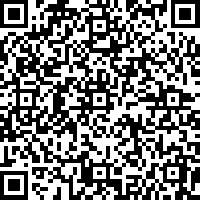
\includegraphics[width=0.7\textwidth]{figure/qrcode.png}
% \end{figure}


\section{Dataset}
\subsection{Dataset Pelatihan Model}
Dataset yang digunakan dalam pengembangan model terdiri dari 2.178 gambar meme yang merupakan gabungan data 	primer dan data sekunder. Untuk mengakses dataset secara lengkap, dapat melalui tautan berikut: \href{https://github.com/elsaelisa09/multimodal-meme-selfharm/tree/main/dataset}{https://github.com/elsaelisa09/multimodal-meme-selfharm/tree/main/dataset}

\subsection{Dataset Pengujian}
Dataset pengujian terdiri dari 19 gambar meme yang berada di luar dataset pelatihan, dengan variasi data eksplisit, implisit, dan ambigu. Untuk mengakses dataset pengujian secara lengkap, dapat melalui tautan berikut: \href{https://github.com/elsaelisa09/multimodal-meme-selfharm/tree/main/Pengujian/Dataset%20Test}{https://github.com/elsaelisa09/multimodal-meme-selfharm/tree/main/Pengujian/DatasetTest}

\section{Anotasi Data}
\subsection{Pedoman Anotasi \textit{Large Language Model}}
Berikut adalah pedoman anotasi yang digunakan untuk LLM dalam proses anotasi data dengan \textit{framework prompt} yang telah disusun mengikuti Rap Guard (\textit{Rationale-aware Defensive Prompting})
\vspace{0.5cm}

\lstset{
	 basicstyle=\ttfamily\small,
	 backgroundcolor=\color{gray!10},
	 frame=single,
	 breaklines=true,
	 columns=fullflexible,
	 showstringspaces=false
}

\begin{lstlisting}
Anda adalah anotator ahli dalam psikologi, dan ahli linguistik.
Tugas Anda adalah mengklasifikasikan meme menjadi [SELF-HARM] atau [NON-SELF-HARM] dengan presisi tinggi.

Sumber Referensi:
1. S.-L. Unterschemmann, E. M. Mueller, S. Lux, A. Philipsen, and M. Schulze, "First evaluation of the emotional picture set of self-injury images (EPSI) using psychophysiological and self-report measures," Borderline Personality Disorder and Emotion Dysregulation, vol. 12, no. 27, 2025. doi: 10.1186/s40479-025-00304-4.
2. J.-W. Guo, J. Kimmel, and L. A. Linder, "Text Analysis of Suicide Risk in Adolescents and Young Adults," Journal of the American Psychiatric Nurses Association, vol. 30, no. 1, pp. 169--173, 2024. doi: 10.1177/10783903221077292.


Langkah 2: Indikator
Berdasarkan analisis relasi di atas, periksa apakah meme ini memenuhi salah satu indikator valid berikut secara ketat:

A. Indikator Narasi & Teks
(1a) Metode dan deskripsi: mendeskripsikan cara menyakiti diri (cutting, burning, overdosis)
(1b) Masking & romantisasi: menganggap self-harm estetik, puitis, atau mekanisme coping yang wajar
(1c) Ideasi bunuh diri: menyiratkan keinginan mati
(1d) Gaslighting/manipulasi: menyalahkan orang lain atas niat menyakiti diri sendiri

B. Indikator Visual dan Simbolik
(2a) Luka fisik: gambar darah, bekas sayatan, lebam
(2b) Alat berbahaya: silet, pisau, tali gantung, tumpukan obat
(2c) Estetika dark humor: gambar ceria/kartun imut tetapi teksnya tentang keinginan mati/bunuh diri (kontras ironis)

Instruksi Label:
Jika terdapat minimal satu indikator terpenuhi (terutama indikator relasional 2c)
-> Klasifikasikan sebagai [SELF-HARM].

Jika tidak ada indikator terpenuhi dan konteks hanya humor umum
-> Klasifikasikan sebagai [NON-SELF-HARM].

Langkah 3: Self-checking
Sebelum memberikan label final, kritik keputusan Anda sendiri:
Apakah saya salah mengartikan slang atau lelucon internet sebagai ancaman serius?
Apakah saya mengabaikan sinyal bahaya terselubung karena gambarnya terlihat lucu (kartun)?

Jika ragu, prioritaskan keselamatan (safety-first approach) namun tetap bedakan
antara dark jokes umum vs promosi self-harm spesifik.
\end{lstlisting}




\subsection{Pedoman Anotasi Data untuk Annotator Manusia}
Berikut adalah pedoman yang harus diikuti oleh anotator manusia dalam melakukan anotasi data dapat diakses pada link berikut: \href{https://github.com/elsaelisa09/multimodal-meme-selfharm/blob/main/dataset/annotation-guideline.pdf}{https://github.com/elsaelisa09/multimodal-meme-selfharm/blob/main/dataset/annotation-guideline.pdf}

\subsection{Lampiran Anotasi Data LLM}
Berikut adalah hasil anotasi data LLM yang dapat diakses pada link berikut : \href{https://github.com/elsaelisa09/multimodal-meme-selfharm/tree/main/Anotasi%20Data%20LLM}{https://github.com/elsaelisa09/multimodal-meme-selfharm/tree/main/AnotasiDataLLM}

\subsection{Lampiran Anotasi Data Manusia}
Berikut adalah lampiran anotasi data yang dilakukan oleh anotator manusia: \href{https://github.com/elsaelisa09/multimodal-meme-selfharm/blob/main/Pengujian/Anotasi%20Manusia%20.xlsx}{https://github.com/elsaelisa09/multimodal-meme-selfharm/blob/main/Pengujian/AnotasiManusia.xlsx}

\section{Kode Program}
\subsection{Kode Program Pelabelan Data LLM}
Berikut adalah kode program yang digunakan untuk melakukan pelabelan data menggunakan LLM dengan pendekatan \textit{framework prompt} yang telah disusun mengikuti Rap Guard (\textit{Rationale-aware Defensive Prompting}). Kode program ini dapat diakses pada link berikut: \href{https://github.com/elsaelisa09/multimodal-meme-selfharm/tree/main/Kode%20Program%20Pelabelan%20Data}{https://github.com/elsaelisa09/multimodal-meme-selfharm/tree/main/KodeProgramPelabelanData}
\subsection{Kode Program Pengembangan dan Pelatihan Model}
Berikut adalah kode program yang digunakan untuk pengembangan dan pelatihan model klasifikasi berbasis multimodal CLIP-ELECTRA dengan pendekatan \textit{intermediate fusion}. Kode program ini dapat diakses pada link berikut: \href{https://github.com/elsaelisa09/multimodal-meme-selfharm}{https://github.com/elsaelisa09/multimodal-meme-selfharm}

